\chapter{Overzicht van gedetailleerde implementatie keuzes}

\begin{figure}[htbf]
\centering
\subfigure[Deployment van HBase met 5 instanties. ]{\label{fig:HBase-deployment}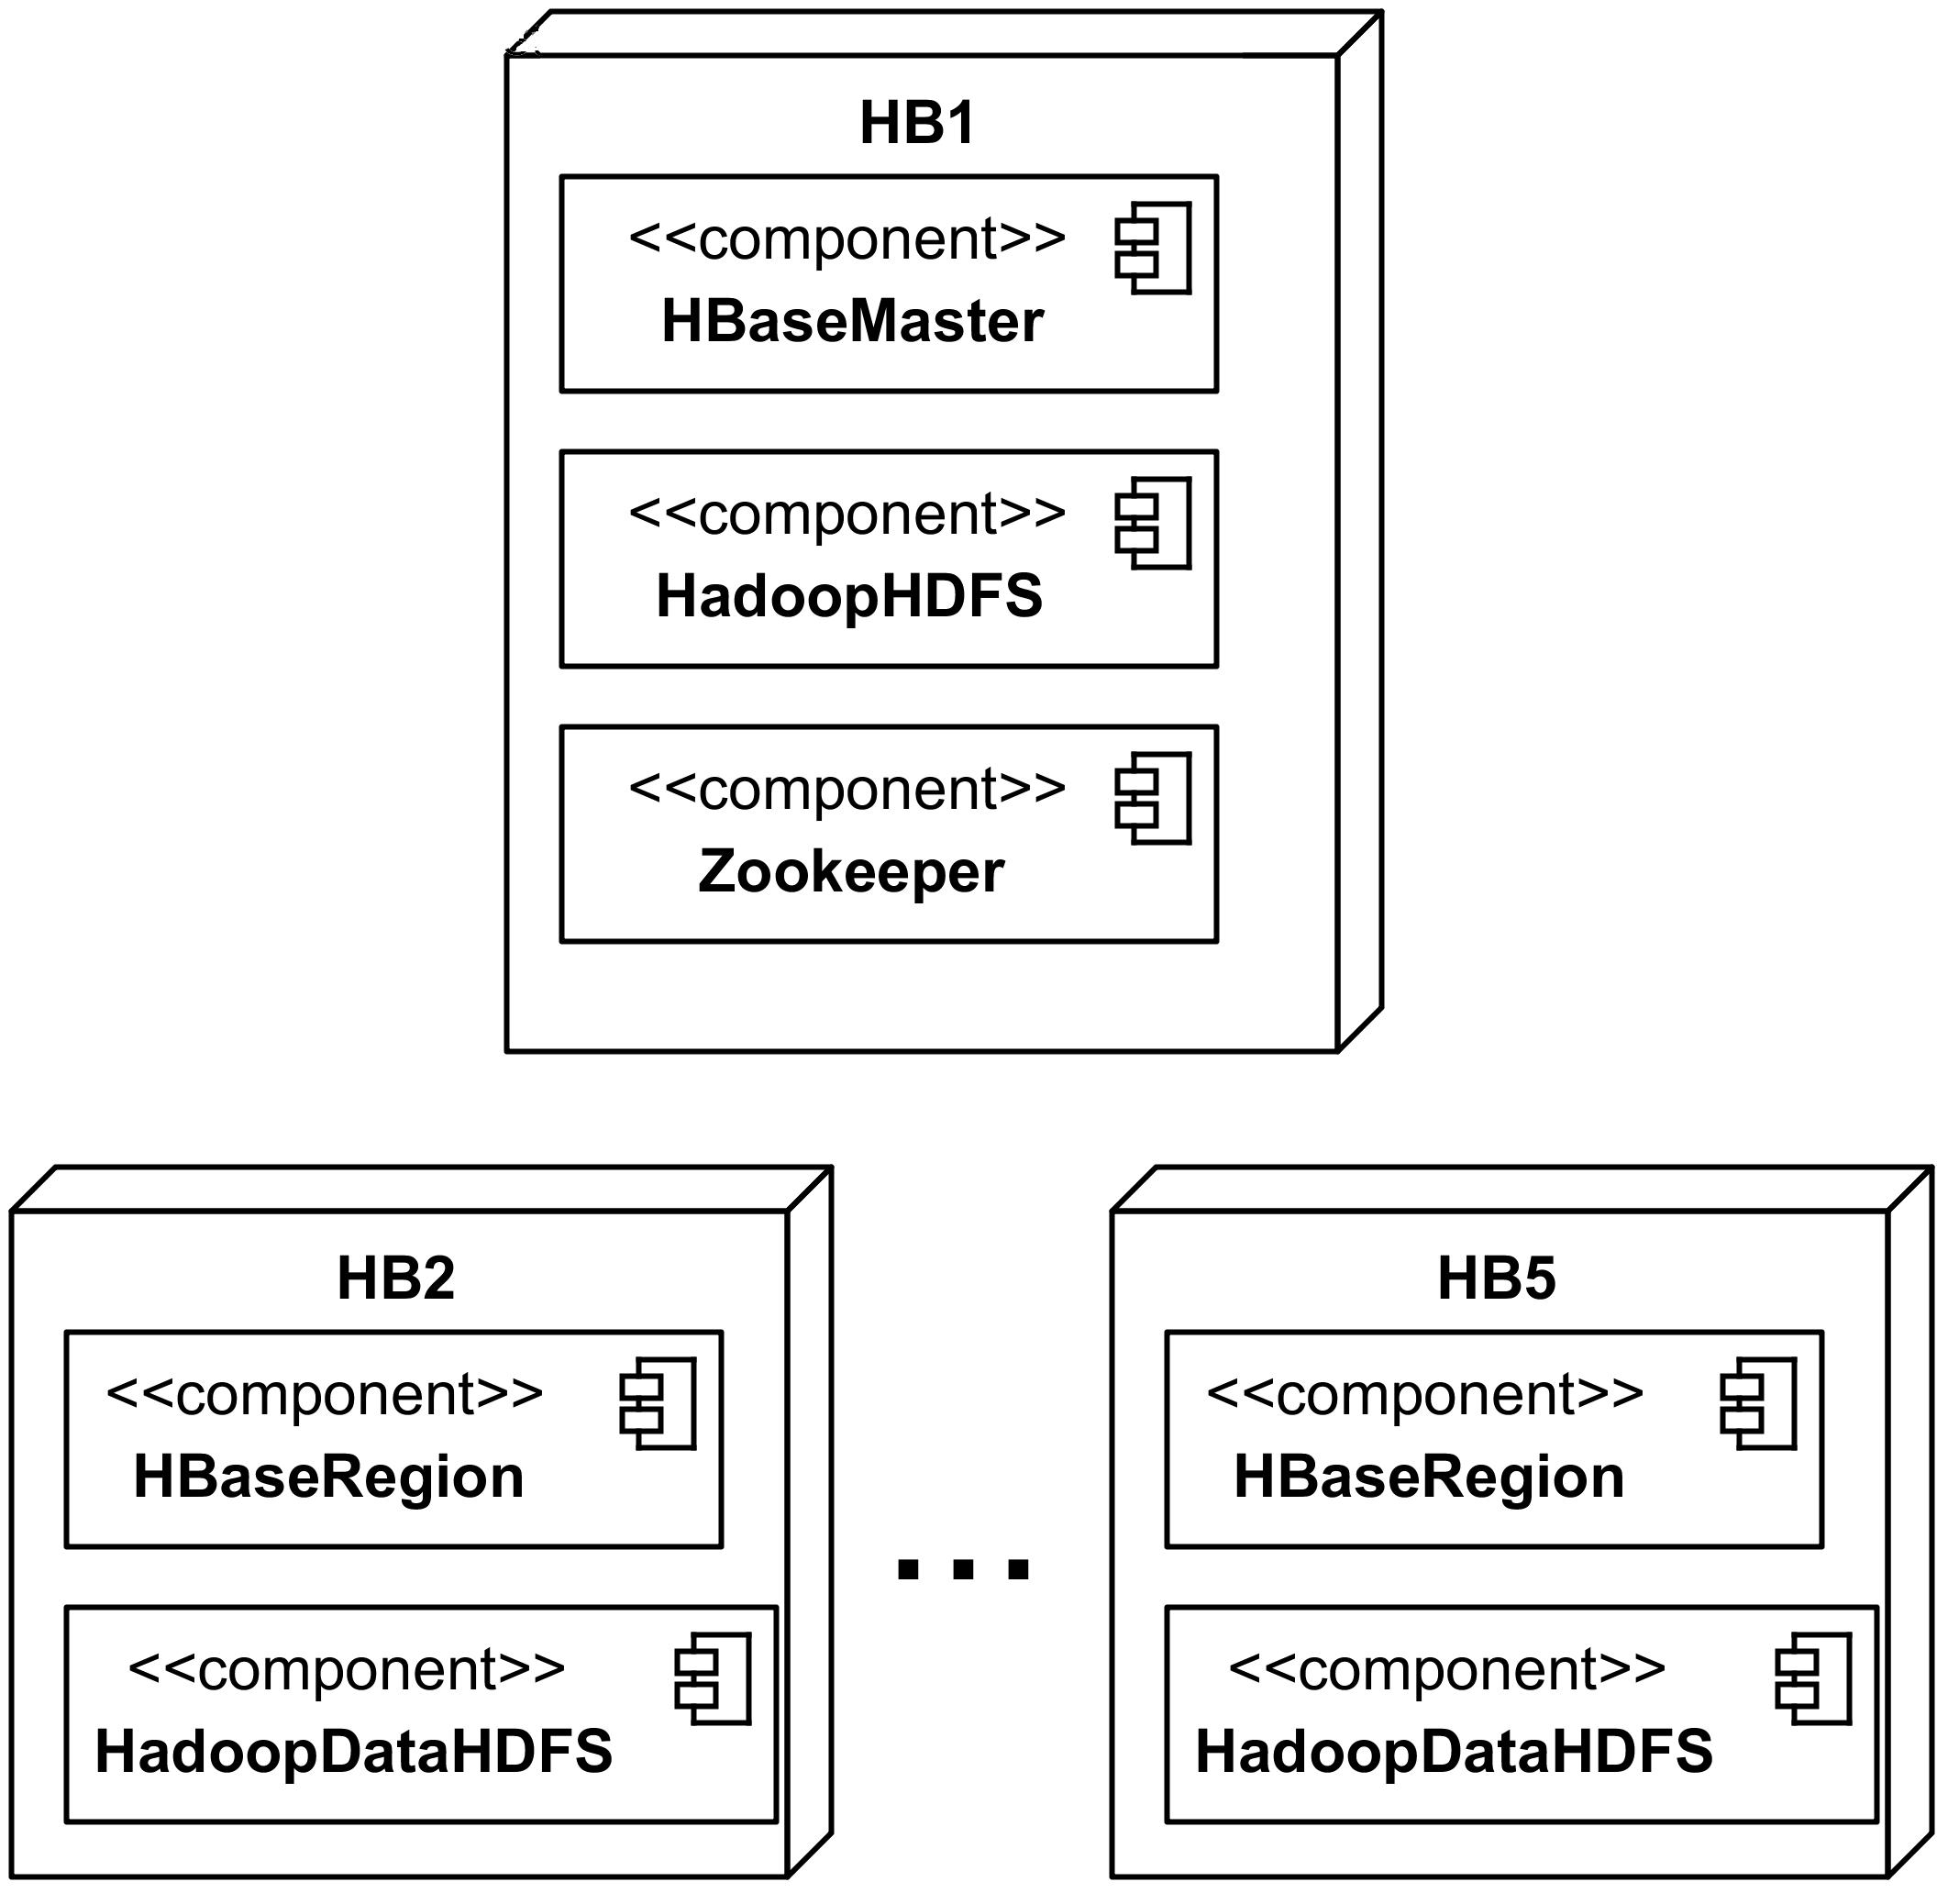
\includegraphics[width=0.55\textwidth]{img/HBase-deployment}}
\subfigure[Deployment van Pgpool-II met 3 instanties. ]{\label{fig:pgpool-deployment}\includegraphics[width=0.35\textwidth]{img/Pgpool-II-deployment}}
\subfigure[Deployment van MongoDB met 6 instanties. ]{\label{fig:MongoDB-deployment}\includegraphics[width=0.65\textwidth]{img/MongoDB-deployment}}
\subfigure[Deployment van de testomgeving met 2 YCSB instanties. ]{\label{fig:YCSB-deployment}\includegraphics[width=0.25\textwidth]{img/YCSB-deployment}}
\caption{Deployment van de verschillende DBMS's en de testomgeving.}\label{fig:deployment-testomgeving}
\end{figure}

\begin{figure}[htbf]

\begin{minipage}[b]{0.4\textwidth}
		\begin{tabular}{l|l}
			\textbf{Naam} & \textbf{eenheid} \\ 
			\hline ID & String \\ 
			Starttijdstip & milliseconden \\ 
			Commando & String \\ 
		\end{tabular} 
	\captionof{table}{Configuratie van event support}
	\label{table:beschikbaarheidinput}
\end{minipage}
\hfill
\begin{minipage}[b]{0.5\textwidth}

\begin{tabular}{l|l}
\textbf{Naam} & \textbf{eenheid} \\ 
\hline ID & String \\ 
Starttijdstip & milliseconden \\ 
Duur van de actie & microseconden \\
Gestart? & Boolean \\
Beëindigd? & Boolean \\
Exit code & Integer 
\end{tabular}
\captionof{table}{Uitvoer van event support}
\label{table:beschikbaarheidoutput}
\end{minipage}
\end{figure}


\begin{table}[htbf]
		\begin{tabular}{L{4cm}|L{2cm}|L{6.5cm}}
			\textbf{Naam} & \textbf{eenheid} & \textbf{Omschrijving} \\ 
			\hline 
			\parbox[t]{4cm}{consistencyTest} & Boolean & \parbox[t]{6.5cm}{Het activeren van de consistentie test}\\ 
			\parbox[t]{4cm}{addSeparateWorkload} & Boolean & \parbox[t]{6.5cm}{Het toevoegen van een basis belasting} \\ 
			\parbox[t]{4cm}{starttime} & \parbox[t]{2cm}{Milli-\newline seconden} & \parbox[t]{6.5cm}{Het startmoment van de consistentie test} \\
			\parbox[t]{4cm}{readThreads} & Integer & \parbox[t]{6.5cm}{Het aantal lees gebruikers} \\ 
			\parbox[t]{4cm}{consistencyDelayMillis} & \parbox[t]{2cm}{Milli-\newline seconden} & \parbox[t]{6.5cm}{Het interval waarin een lees gebruiker opnieuw het record leest} \\ 
			\parbox[t]{4cm}{newrequestperiodMillis} & \parbox[t]{2cm}{Milli-\newline seconden} & \parbox[t]{6.5cm}{Het interval waarin een schrijf gebruiker opnieuw een record schrijft} \\ 
			\parbox[t]{4cm}{insertProportion- \newline ConsistencyCheck} & \parbox[t]{2cm}{Float \newline ($0\leq x \leq 1)$} & \parbox[t]{6.5cm}{Het percentage van schrijfacties dat een nieuw record invoegt} \\ 
			\parbox[t]{4cm}{updateProportion- \newline ConsistencyCheck} & \parbox[t]{2cm}{Float \newline ($0\leq x \leq 1)$} & \parbox[t]{6.5cm}{Het percentage van schrijfacties dat een record aanpast} \\ 
			\parbox[t]{4cm}{stopOnFirstConsistency} & Boolean & \parbox[t]{6.5cm}{Stop zodra de eerste keer een correct record is gelezen} \\ 
			\parbox[t]{4cm}{maxDelayConsistency- \newline BeforeDropInMicros} & \parbox[t]{2cm}{Micro-\newline seconden} & \parbox[t]{6.5cm}{De maximale afwijking tussen de eigenlijke start van de query en het geplande moment} \\ 
			\parbox[t]{4cm}{timeoutConsistency- \newline BeforeDropInMicro} & \parbox[t]{2cm}{Micro-\newline seconden} & \parbox[t]{6.5cm}{De maximale tijd dat een leesactie geprobeerd wordt}\\
		\end{tabular} 
	\captionof{table}{Configuratie van de consistentie testen}
	\label{table:consistentieinput}
\end{table}

\begin{table}[htbf]
\centering
		\begin{tabular}{l|l|l}
			\textbf{Naam} & \textbf{eenheid} & \textbf{Omschrijving} \\ 
			\hline Tijd & Microseconden & Het moment dat de schrijfactie moest starten\\ 
			GebruikersID & R/W-Integer & Het id van de gebruiker (W-0, R-0, R-1, ..) \\ 
			Start & Microseconden & Het moment dat actie is begonnen \\
			Vertraging & Microseconden & De tijd dat de actie heeft geduurd \\ 
			Waarde & String & De gelezen of geschreven waarde \\ 
		\end{tabular} 
	\captionof{table}{Uitvoer van een enkel query in de consistentie testen}
	\label{table:consistentieuitvoer}
\end{table}

\begin{table}[htbf]
	\centering
		\begin{tabular}{l|l}
			\multicolumn{2}{c}{\textbf{Stoppen}} \\
			\textbf{Wat} & \textbf{Commando} \\ 
			\hline
			Zachte stop & service \{\{service-name\}\} stop \\ 
			Harde stop & kill -KILL \{\{process Id\}\} \\ 
			Netwerk onderbreken & iptables -A OUTPUT -d 0.0.0.0/0 -j DROP  \\ 
			\multicolumn{2}{c}{~} \\
			\multicolumn{2}{c}{\textbf{Heropstarten}} \\
			\textbf{Wat} & \textbf{Commando} \\ 
			\hline
			Zachte start & service \{\{service-name\}\} restart \\ 
			Harde start & service \{\{service-name\}\} restart \\ 
			Netwerk herstellen & iptables -D OUTPUT 1  \\ 
			\multicolumn{2}{c}{~}  \\
			\multicolumn{2}{c}{\textbf{Speciale commando's}} \\
			\textbf{Wat} & \textbf{Commando} \\ 
			\hline
			Pgpool-II & /usr/local/bin/pcp\_recovery\_node -d 10 \{\{pgpool host\}\} \{\{port\}\} \\
			\hspace*{0.5cm} (Online recovery) &  \hspace*{0.5cm} \{\{gebruikersnaam\}\} \{\{wachtwoord\}\}  \{\{node nummer\}\} \\
		\end{tabular} 
	\captionof{table}{Beschikbaarheidstesten: Overzicht van de commando's voor het stoppen en starten in de verschillende modes. }
	\label{table:beschikbaarheidstesten-commandos}
\end{table}